%--------------------------------------------
% Chapter: PROJECT GOALS
%--------------------------------------------
\chapter{Project's context and goals}
\label{sec:projGoals}

The very first target was to adapt a new hardware (Raspberry Pi) including a autonomous landing to the Quadrocopter from Hochschule Esslingen (HElikopter). As this was not enough work for all of us, the project was extended to include a autonomous landing, too. We were a team of 4 students who were interested in a project work with the HElikopter. We internally agreed in splitting the work in 2 parts. The other two students were more interested in developing the new hardware platform and software and we liked to care about the autonomous landing.

As we developed the autonomous landing to the new hardware, there was a slight dependence to each other.
Following are the goals:
\begin{itemize}
	\item Autonomous Landing
	\item Effective Distance measurement to ground
	\item Implementation on Raspberry Pi
\end{itemize}

This document describes a project in the context of the curriculum's module 'project work' of the masters program Software-based Automotive Systems. The project intends to set up a generic hardware and software platform to control the HElikopter Quadrocopters of Hochschule Esslingen, Faculty Information Technology. The platform shall be based on a real-time capable Linux Operating System and a Raspberry Pi B+ Board. Furthermore, all components used shall be available on market as much ready-made as possible.

Originally, the project was designed to be elaborated by a group of four students. Unfortunately, two students had to face some substantial problems during the project work. Eventually, the project got split up into two separated groups. In consequence, the initially intended goals could not be reached completely. This is partly reflected in the below shown tasks, milestones and project goals.

\begin{figure}[h]
    \centering
    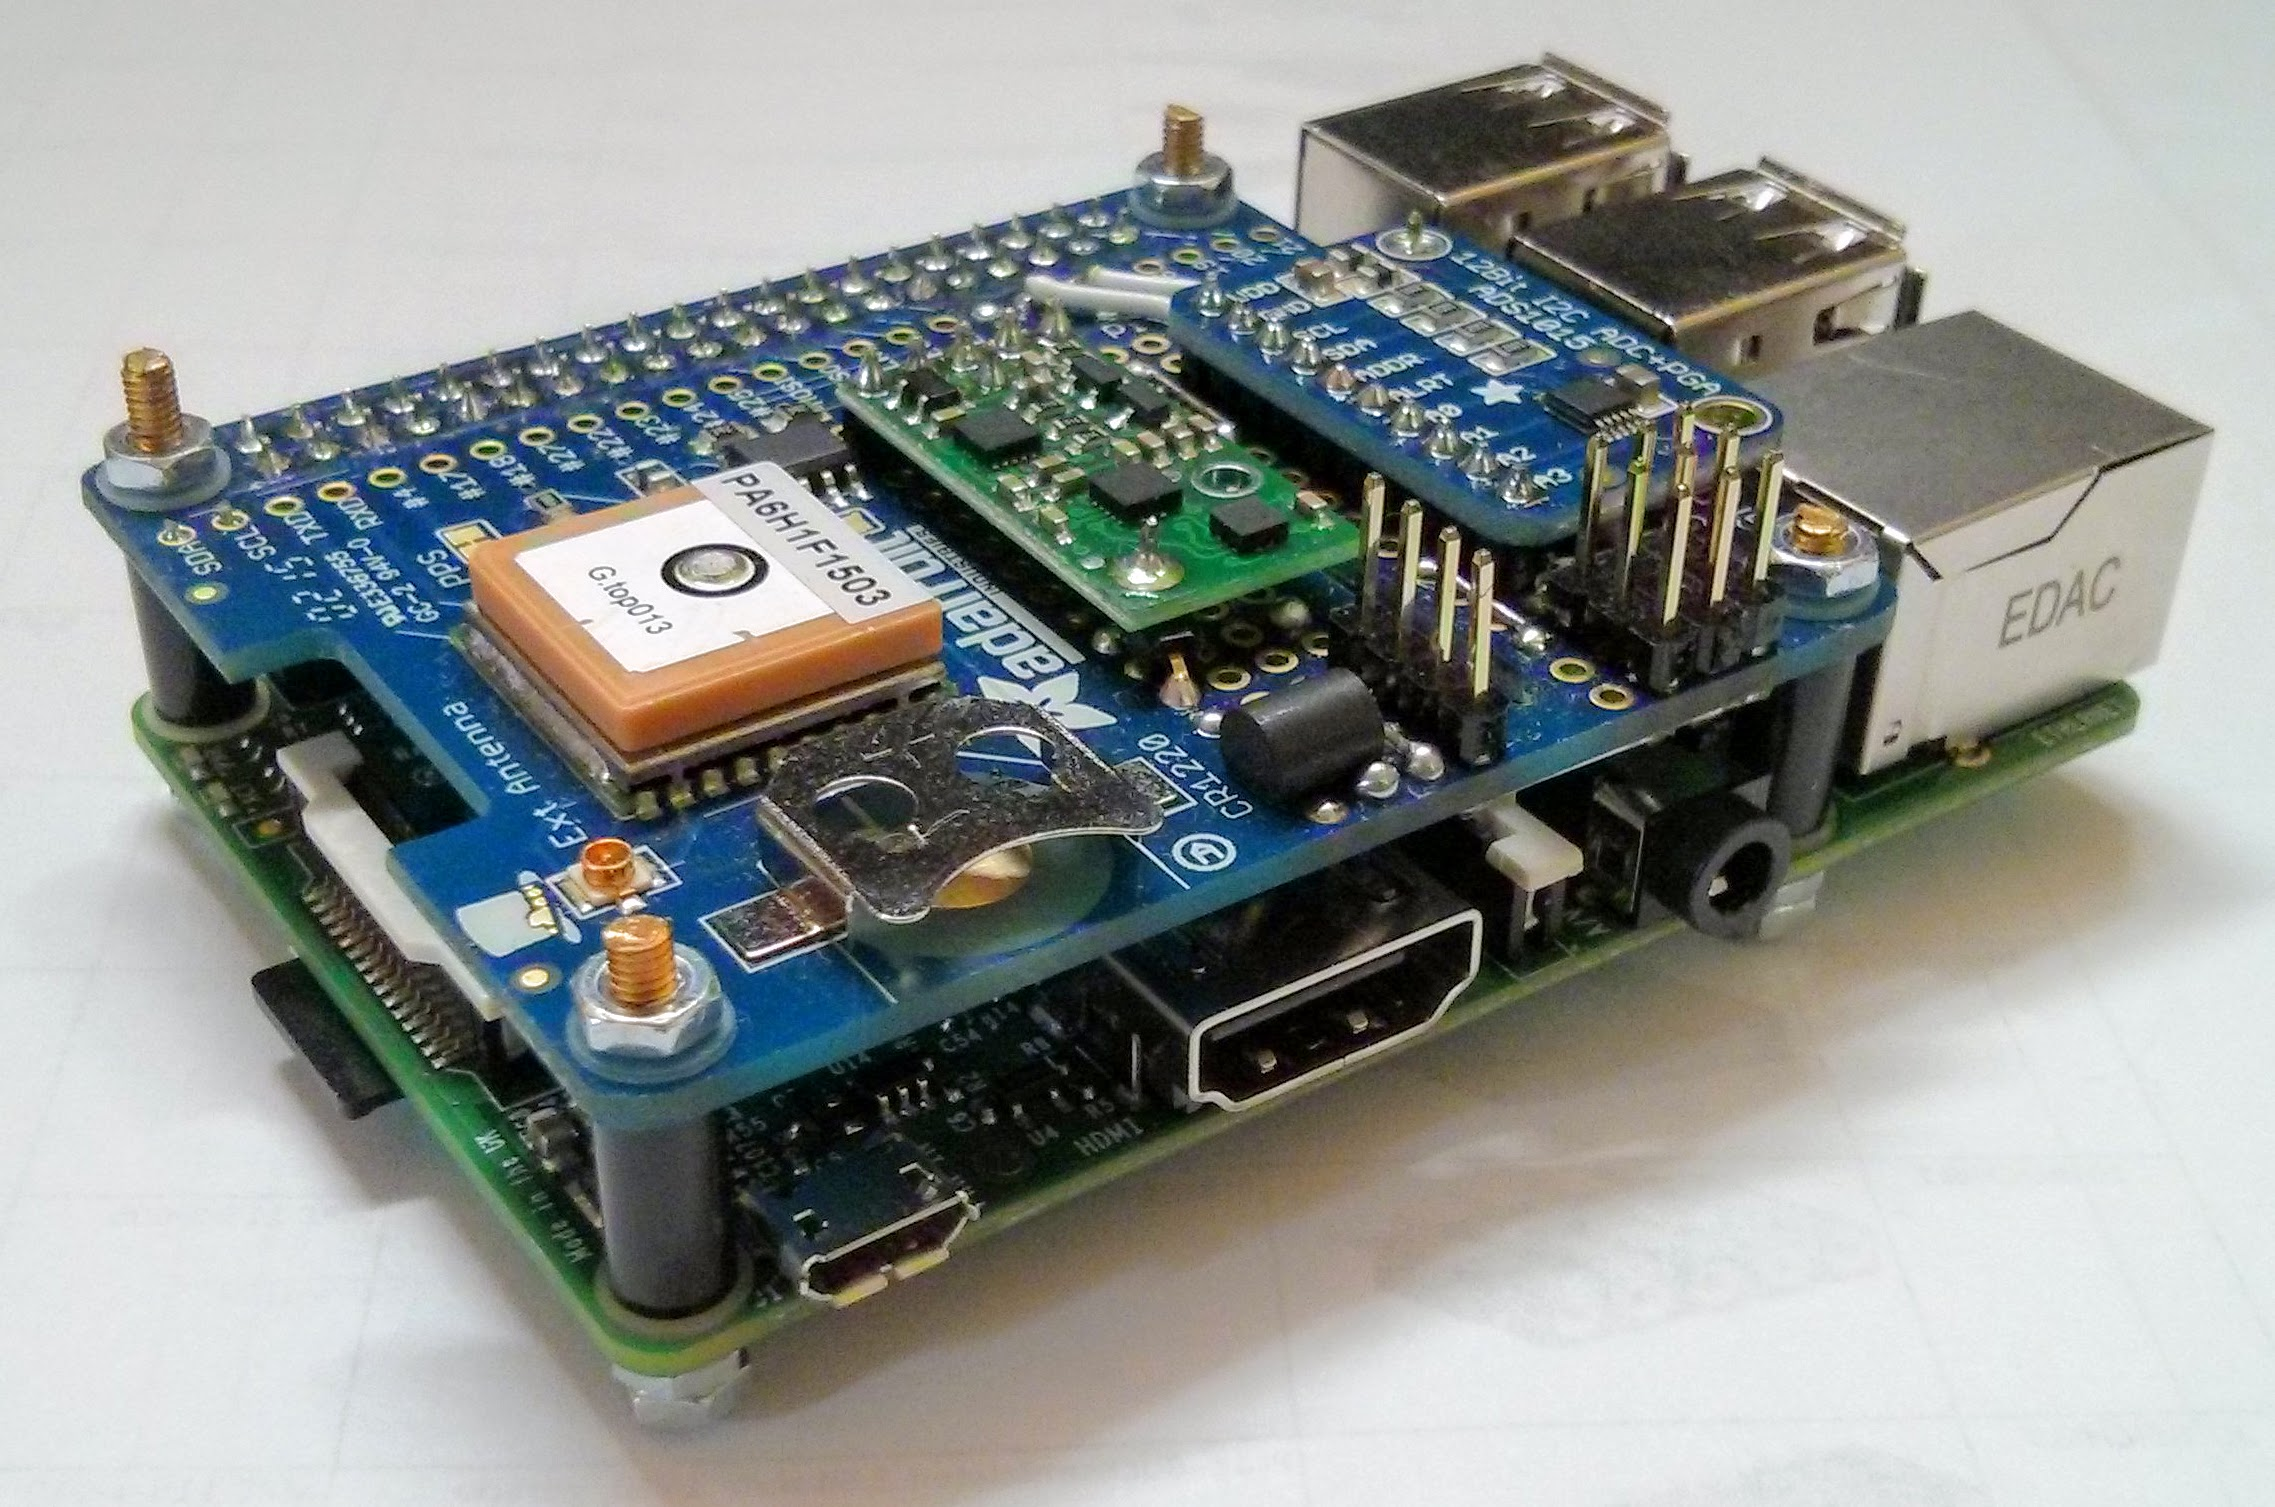
\includegraphics[width=0.85\textwidth]{fig/ch-project-goals/MainRaspberryPi}
    \caption{Raspberry Pi based Quadrocopter Platform (Controller Board)}
    \label{fig:projGoals:RpiPic}
\end{figure}

Nevertheless, the authors of this document are confident that the shown Raspberry Pi based platform is a solid and stable approach. With some extensions on this work, a Linux-driven Quadrocopter can be realized in a future project work.

%- - - - - - - - - - - - - - - - - - - - - - 
% Section: Temporal project scope
%- - - - - - - - - - - - - - - - - - - - - - 
\section{Temporal project scope}
\label{sec:projGoals:temporalProj}
The project started in \textbf{March 23, 2015} and ended in \textbf{June 26, 2015}.

The following milestones were initially set up:
\begin{table}[H]	
	\begin{tabular}{|c|c|c|c|}
\hline
&&&\\
\textbf{Nr.} & \textbf{Date} & \textbf{Milestone's goal} & \textbf{Status}\\
&&&\\
\hhline{|=|=|=|=|}
&&&\\
	1 & April 1, 2015 & Hardware selected & \textcolor[rgb]{0,0.58,0}{\textbf{successfully reached}}\\
	&&&\\
\hline
&&&\\
				2 & May 11, 2015 & HAL drivers finalized& \textcolor[rgb]{0,0.58,0}{\textbf{successfully reached}}\\
				&&&\\
\hline
&&&\\
				3 & May 25, 2015&First prototyp with flying capabilities& \textcolor[rgb]{1,0.41,0.13}{\textbf{partly reached}}\\
				&&&\\
\hline
&&&\\
				4 & June 15, 2015& First prototyp with position hold &\textcolor[rgb]{1,0,0}{\textbf{not reached}}\\
				&&&\\
\hline
	\end{tabular}
	\caption{Initially set up milestones for the project MasterQuad 2015}
	\label{tab:projGoals:milestones}
\end{table}
%\begin{enumerate}
	%\item \textbf{Milestone}: \textcolor[rgb]{0,0.58,0}{(\textbf{successfully reached})}\\
				%\textbf{Date}: April 1, 2015\\
				%\textbf{Goal}: Hardware selected
	%\item \textbf{Milestone}: \textcolor[rgb]{0,0.58,0}{(\textbf{successfully reached})}\\
				%\textbf{Date}: May 11, 2015\\
				%\textbf{Goal}: HAL drivers finalized
	%\item \textbf{Milestone}: \textcolor[rgb]{1,0.41,0.13}{(\textbf{partly reached})}\\
				%\textbf{Date}: May 25, 2015\\ 
				%\textbf{Goal}: First prototyp with flying capabilities
				%
	%\item \textbf{Milestone (optional)}: \textcolor[rgb]{1,0,0}{(\textbf{not reached})}\\
				%\textbf{Date}: June 15, 2015\\
				%\textbf{Goal}: First prototyp with position hold
%\end{enumerate}

%- - - - - - - - - - - - - - - - - - - - - - 
% Section: Contentual project scope
%- - - - - - - - - - - - - - - - - - - - - - 
\section{Contentual project scope}
\label{sec:projGoals:projPlan:cententual}
The original project goals where defined as followed:
\begin{enumerate}
	\item Select new hardware (Raspberry-based with Linux capability) 
	\item Setting up RTOS (Preempt RT Kernel)
	\item Writing HAL drivers for new Hardware
	\item Writing a sensor fusion for orientation filtering and signal enhancement
	\item Integrate existing control software (if possible)
	\item Setup of flight model to simulate position hold
	\item Implement controllers for position hold
\end{enumerate}

Not all goals could be successfully reached - items 5 to 7 could not be completely realized within the project time. Nevertheless, a stable and performant core system has been set up that can be utilized for further projects and applications.

%- - - - - - - - - - - - - - - - - - - - - - - 
% Section: Tasks and responsible team members
%- - - - - - - - - - - - - - - - - - - - - - - 
\section{Tasks and responsible team members}
\label{sec:projGoals:tasksAndMembers}

\textemphs{Oliver Breuning} (E-Mail: olbrgs00@hs-esslingen.de)

Responsibilities:
\begin{itemize}
	\item Virtual Machine as Development Environment (see Chapter \ref{sec:sec-VM})
	\item Low-Level-Driver for UART access
	\item HAL-Driver for battery check
	\item HAL-Driver for GPS
	\item HAL-Driver for Barometer
	\item HAL-Driver for Gyroscope
	\item Generic Library for fast Matrix-Operations
	\item Sensor-Fusion for IMU (see Chapter \ref{sec:sensorFusion})
	\item Tilt-compensation for Intertial Measurement Unit (IMU) (see Chapter \ref{sec:angle})
	\item Complementary-Filter (see Chapter \ref{sec:ComplementaryFilter})
	\item Kalman-Filter (see Chapter \ref{sec:KalmanFilter})
\end{itemize}

\vspace{0.5cm}

\textemphs{J\"urgen Schmidt} (E-Mail: juscgs00@hs-esslingen.de)

Responsibilities:
\begin{itemize}
	\item Project management
	\item Hardware layout and mechanical packaging
	\item Software architecture and layout
	\item HAL-Driver for Accelerometer
	\item HAL-Driver for Magnetometer
	\item Live network connection for MATLAB (UDP-based)
	\item Linux Kernel update with PREEMPT\_RT patch
	\item Kernel module for precise PPM measurement
	\item Kernel module for precise time trigger control (unstable yet!)
\end{itemize}


\begin{figure}[H]
    \centering
    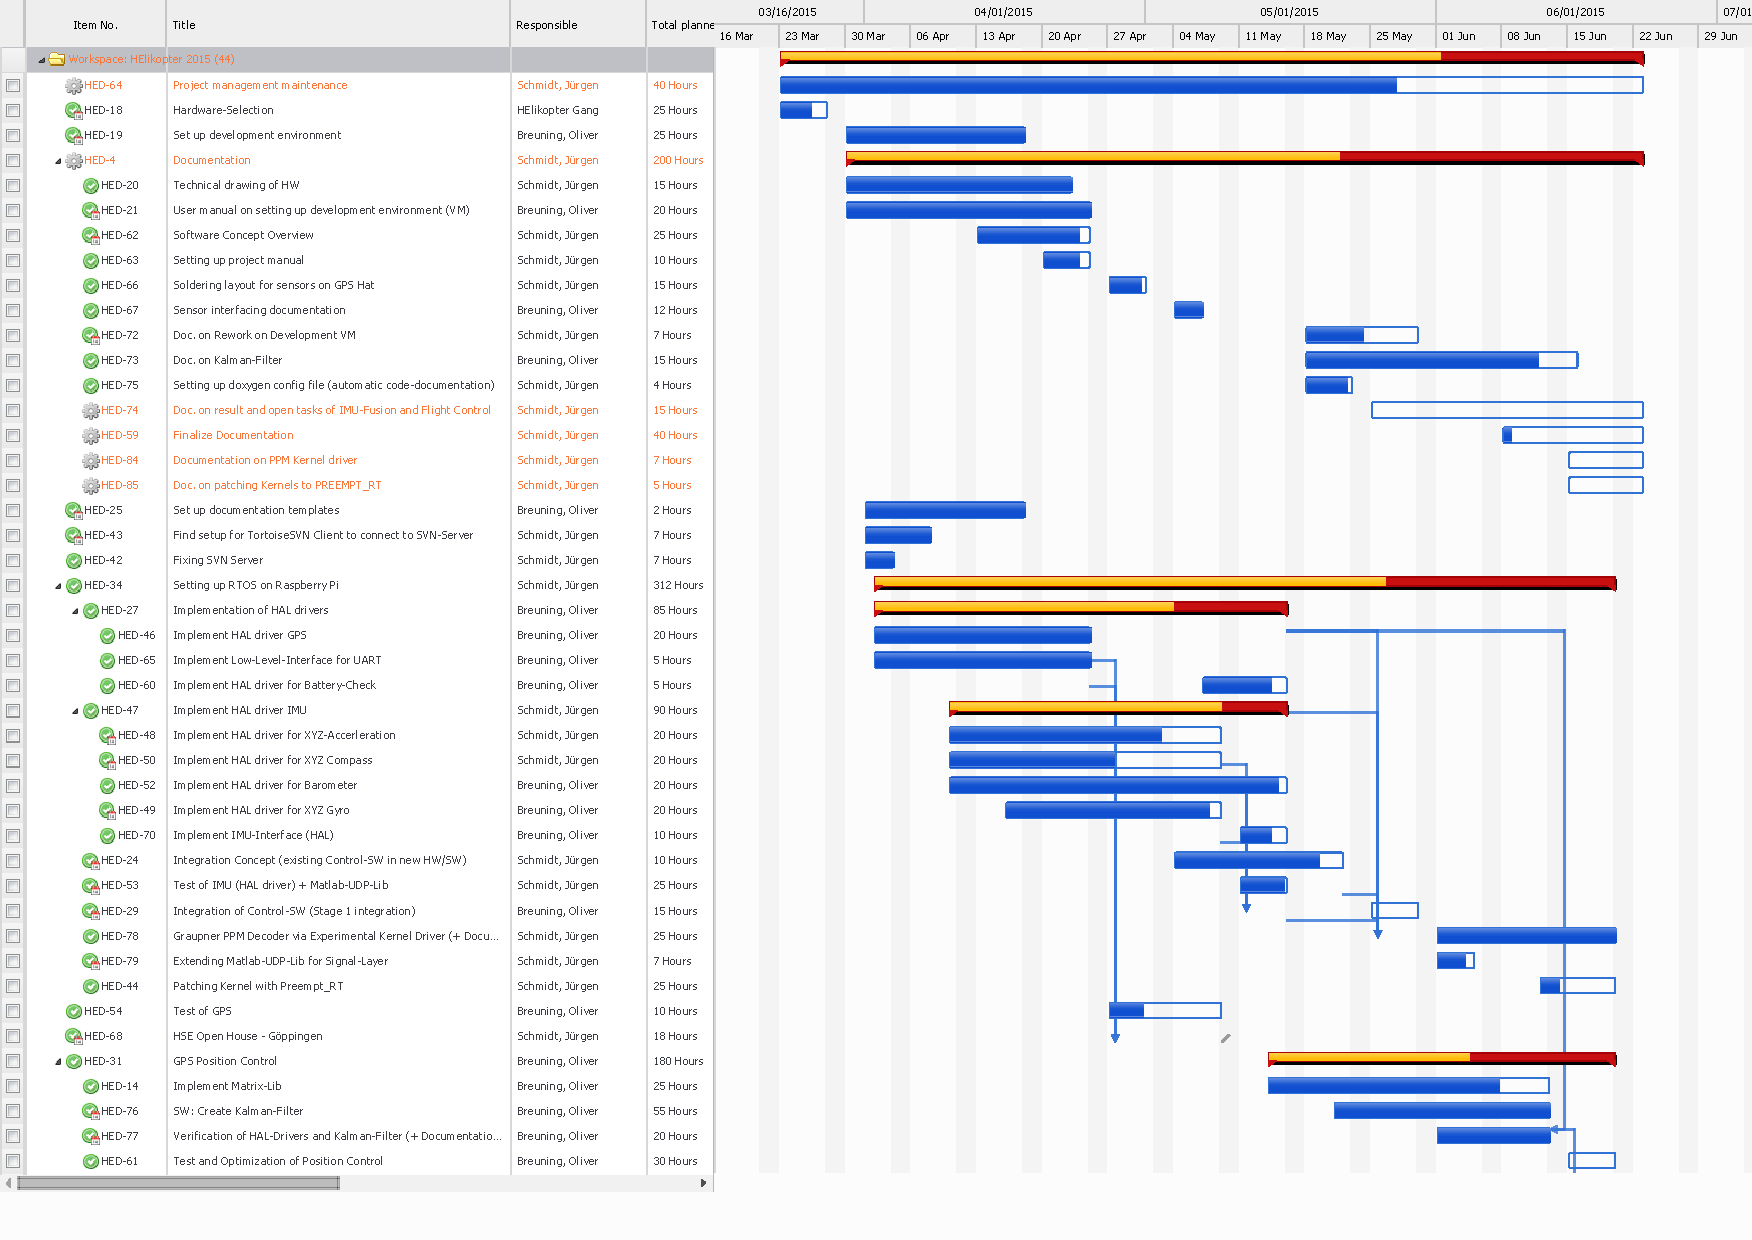
\includegraphics[angle=90,width=\textwidth]{fig/ch-project-goals/project_plan}
    \caption[Gantt diagram of project MasterQuad 2015 (Track+)]{Gantt diagram of the project plan of MasterQuad 2015 (Track+ output)}
    \label{fig:projGoals:ganttDiagram}
\end{figure}

%- - - - - - - - - - - - - - - - - - - - - - - 
% Section: Repository structure
%- - - - - - - - - - - - - - - - - - - - - - - 
\section{Repository structure}
\label{sec:projGoals:repos}

For version controlling, the subversion system of the HElikopter Project has been used. Every team member has regarded the following given folder structure in order to keep a structured and organized working flow.
\dirtree{%
.1 /.
.2 doc\DTcomment{\textbf{Finalized documentation}}.
.3 pm\DTcomment{Documentation regarding project management}.
.4 meetings\DTcomment{Meeting reports and meeting template}.
.4 sources\DTcomment{LaTex sources of all documents in \texttt{/doc/pm}}.
.3 se\DTcomment{Documentation regarding system engineering}.
.4 sources\DTcomment{LaTex sources of all documents in \texttt{/doc/se}}.
.2 impl\DTcomment{\textbf{Source code}}.
.3 branch\DTcomment{Container for parallel development lines to trunk}.
.3 tag\DTcomment{Finalized and stable software}.
.3 trunk\DTcomment{Current development line}.
.4 app\DTcomment{Application Layer Software}.
.4 doc\DTcomment{Automatic code documentation via Doxygen}.
.4 hal\DTcomment{Hardware Abstraction Layer Software}.
.4 kern\DTcomment{Custom Linux Kernel modules}.
.4 matlab\DTcomment{Network connection to MATLAB}.
.4 sig\DTcomment{Signal Processing Layer Software}.
.2 scratch\DTcomment{\textbf{Documents or files in progress, excluding source code}}.
.3 doc\_template\DTcomment{Templates for documentation files (mainly LaTex)}.
.2 sys\DTcomment{\textbf{Firmwares, OS and development environment}}.
.3 RPi\DTcomment{Preconfigured firmware(s) for Raspberry Pi B+}.
.3 VM\DTcomment{Development Environment VM with all IDEs preconfigured}.
}

Within the folders 
\begin{itemize}
	\item \texttt{/impl/trunk/app}
	\item \texttt{/impl/trunk/hal}
	\item \texttt{/impl/trunk/sig}
\end{itemize}
a subfolder for each functional unit shall be created. The functional units shall be considered as depicted in figure \ref{fig:layer:layer_graph} (smaller boxes inside of the colored layers). Example:
\dirtree{%
.1 /.
.2 impl.
.3 trunk.
.4 hal.
.5 adc.
.5 gps.
.5 gyro.
}

\subsection*{Storing test files}
\label{sec:work:groupware:test}
For each software component, a separate test should be written to ensure the software quality. All source code files and test data files to run a test shall be saved in a separate subfolder named \texttt{tst}. Example:
\dirtree{%
.1 /.
.2 impl.
.3 trunk.
.4 hal.
.5 gps.
.6 tst\DTcomment{contains data \& code to test the module 'gps'}.
.7 test\_data.dump.
.7 helper\_code.c.
.7 helper\_code.h.
.7 test\_main.c.
.6 gps.c\DTcomment{actual source of module 'gps'}.
.6 gps.h\DTcomment{actual interfaces of module 'gps'}.
}


\textbf{Important note:}\\
The \texttt{tst}-folder will \textbf{not} be moved to the tags folders! All data in \texttt{/imp/tags} is considered to be well tested and stable. Therefore, the test data is not required to move.

%--------------------------------------------
% section: DOCUMENTATION
%--------------------------------------------
\section{Documentation}
\label{sec:work:docu}
The project team delivered the following documents:
\begin{itemize}
	\item Project manual (\texttt{/doc/pm})
	\item Technical drawings of hardware (\texttt{/doc/se}, see also chapter \ref{sec:hardware:techDrawAndPack})
	\item Bill of materials (\texttt{/doc/se}, see also chapter \ref{sec:hardware:BillOfMat})
	\item Software structure \& concept (\texttt{/doc/se}, see also chapter \ref{sec:software})
	\item User manual of project (this document)
	\item Doxygen-based code documentation (see appendix \ref{sec:b-codeDoc})
\end{itemize}

The doxygen-based code documentation is delivered in the SVN repository as HTML output of the current working copy. The doxygen configuration file has been submitted in \texttt{/impl/trunk/doc/} (see also Appendix \ref{sec:b-codeDoc}). To regenerate the code documentation to the latest version, run \texttt{doxygen} in the above mentioned folder.